% =====================================================================
%  MASTER FILE — Smart Automated Protein Shake Vending Machine Thesis
%  Overleaf-compatible. Compile with pdfLaTeX + BibTeX (IEEEtran style).
%  Each new chapter is added as \input{chapterN} below; the ToC and
%  bibliography grow automatically — nothing is ever overwritten.
% =====================================================================
\documentclass[12pt,a4paper,oneside]{report}

% ---------- Core packages ----------
\usepackage[utf8]{inputenc}
\usepackage[T1]{fontenc}

\usepackage[margin=2.5cm]{geometry}
\usepackage{amsmath,amssymb,amsfonts}
\usepackage{graphicx}
\usepackage{booktabs}
\usepackage{longtable}
\usepackage{array}
\usepackage{caption}
\usepackage{subcaption}
\usepackage{siunitx}
\usepackage{enumitem}
\usepackage[expansion=false]{microtype} % expansion off: bitmap CM fonts in this distro
\usepackage[hidelinks]{hyperref}

% ---------- Diagram packages (used throughout the thesis) ----------
\usepackage{tikz}
\usetikzlibrary{arrows.meta,automata,positioning,shapes.geometric,
                shapes.multipart,calc,fit,backgrounds,decorations.pathreplacing}
\usepackage{circuitikz}   % electronics chapters
\usepackage{pgfplots}     % data/plots chapters
\pgfplotsset{compat=1.18}

% ---------- Code listings (payment webhook, firmware, controller) ----------
\usepackage{listings}
\usepackage{xcolor}
\definecolor{codebg}{RGB}{248,248,248}
\definecolor{codekw}{RGB}{0,60,150}
\definecolor{codestr}{RGB}{150,60,0}
\definecolor{codecmt}{RGB}{90,120,90}
\lstset{
  backgroundcolor=\color{codebg},
  basicstyle=\ttfamily\footnotesize,
  keywordstyle=\color{codekw}\bfseries,
  stringstyle=\color{codestr},
  commentstyle=\color{codecmt}\itshape,
  numbers=left, numberstyle=\tiny, numbersep=6pt,
  frame=single, framerule=0.3pt, breaklines=true,
  showstringspaces=false, tabsize=2, captionpos=b
}

% ---------- IEEE-style citations ----------
\usepackage{cite}                 % [1]–[3] compression

% ---------- Numbering conventions (consistent across all chapters) ----------
\numberwithin{equation}{chapter}
\numberwithin{figure}{chapter}
\numberwithin{table}{chapter}

% ---------- Global TikZ styles reused by every chapter ----------
\tikzset{
  sysstate/.style={rectangle, rounded corners=3pt, draw=black, thick,
                   minimum width=3.1cm, minimum height=0.95cm,
                   align=center, font=\small, fill=blue!6},
  errstate/.style={sysstate, fill=red!10, draw=red!60!black},
  okstate/.style={sysstate, fill=green!10, draw=green!50!black},
  decision/.style={diamond, aspect=2.2, draw=black, thick, align=center,
                   font=\small, fill=yellow!12, inner sep=1pt},
  layerbox/.style={rectangle, rounded corners=4pt, draw=black, thick,
                   minimum width=12.6cm, minimum height=1.7cm,
                   align=center, font=\small},
  modbox/.style={rectangle, draw=black!70, thin, rounded corners=2pt,
                 minimum width=2.55cm, minimum height=0.8cm,
                 align=center, font=\scriptsize, fill=white},
  flow/.style={-{Stealth[length=2.6mm]}, thick},
  busflow/.style={{Stealth[length=2.4mm]}-{Stealth[length=2.4mm]}, thick, dashed}
}

% =====================================================================
\begin{document}

% ---------- Front matter ----------
\begin{titlepage}
  \centering
  \vspace*{2.5cm}
  {\LARGE\bfseries Design and Development of an IoT-Based Smart Automated
   Protein Shake Vending Machine\par}
  \vspace{0.6cm}
  {\large with Cashless Payment, Refrigerated Water System, Precision Powder
   Dispensing, and Automatic Cup Dispensing\par}
  \vspace{2.2cm}
  {\large A Commercial-Grade Engineering Thesis\par}
  \vfill
  {\large \today\par}
\end{titlepage}

\tableofcontents
\listoffigures
\listoftables
\clearpage

% ---------- Chapters (append one line per chapter as we progress) ----------
% =====================================================================
%  CHAPTER 1 — System Overview & User Workflow
%  Cited keys live in references.bib (Chapter 1 block).
% =====================================================================
\chapter{System Overview and User Workflow}
\label{ch:overview}

\section{Introduction}
\label{sec:intro}

Automated retail has evolved from simple gravity-drop snack machines into
mechatronic systems that prepare a product on demand. Freshly prepared
beverages are the most demanding category in this space: unlike packaged
goods, a made-to-order protein shake requires the machine to \emph{measure},
\emph{combine}, \emph{mix}, and \emph{serve} consumable ingredients within a
strict hygiene envelope, while simultaneously handling money, inventory, and
remote telemetry. The machine developed in this thesis --- an IoT-based smart
automated protein shake vending machine --- therefore sits at the
intersection of four engineering domains:

\begin{enumerate}[itemsep=2pt]
  \item \textbf{Precision mechatronics:} gravimetric powder dosing to
        \SI{\pm 1}{\gram} across serving sizes of \SI{30}{\gram},
        \SI{45}{\gram}, and \SI{60}{\gram}, using closed-loop auger
        metering against HX711-instrumented load cells~\cite{hx711datasheet}.
  \item \textbf{Thermal-fluid engineering:} a refrigerated liquid subsystem
        holding water at \SIrange{4}{8}{\celsius} and a separately
        refrigerated milk circuit, with clean-in-place provisions.
  \item \textbf{Embedded and distributed control:} a Raspberry~Pi~5
        orchestrator~\cite{rpi5brief} coordinating ESP32 actuator
        nodes~\cite{esp32datasheet} over MQTT~\cite{oasis2019mqtt}, an
        architecture chosen so that hard-real-time motor control is
        physically separated from the soft-real-time UI and network stack.
  \item \textbf{Fintech integration:} fully cashless operation over
        UPI~\cite{npci_upi}, QR, NFC, and card rails compliant with EMV
        contactless~\cite{emvco_contactless} and PCI~DSS~\cite{pcidss4}
        handling constraints.
\end{enumerate}

This chapter defines the problem, states the design objectives, and then
develops the artifact that every subsequent chapter is anchored to: the
\emph{complete user workflow}, formalized as a finite-state machine in the
statechart tradition of Harel~\cite{harel1987statecharts}, together with the
three-layer system architecture (UI / payment / control) presented at block
level. Chapters 2--4 each expand one layer of this architecture; Chapters
5--9 expand the electromechanical plant that the control layer drives.

\section{Background and Motivation}
\label{sec:background}

Gyms, university campuses, and corporate fitness centers exhibit a demand
pattern that conventional retail serves poorly: short, sharp bursts of
identical purchases (post-workout shakes) concentrated in narrow time
windows. Staffed shake bars are labor-inefficient at this duty cycle;
pre-bottled shakes sacrifice freshness, temperature, and formulation choice.
An unattended machine that prepares a chilled, freshly mixed shake in under
a minute addresses this gap --- but only if it solves three problems that
have historically kept powder-based beverage vending niche:

\begin{description}[itemsep=2pt]
  \item[Dosing repeatability.] Protein powders are cohesive, hygroscopic,
    and prone to bridging and ratholing in hoppers. Open-loop volumetric
    dosing drifts as bulk density changes with humidity and fill level;
    the design must therefore be \emph{gravimetric} (weight-feedback) rather
    than volumetric. This drives the ESP32~+~HX711 closed-loop node design
    detailed in Chapter~6.
  \item[Hygiene of the wet path.] Milk and reconstituted protein are
    high-risk media for microbial growth. Every wetted component must be
    designed for automated rinse cycles and scheduled sanitation consistent
    with HACCP principles~\cite{codexhaccp}, ISO~22000~\cite{iso22000}, and
    vending-specific requirements such as NSF/ANSI~25~\cite{nsf25}
    (Chapters~7, 8, and~11).
  \item[Unattended trust.] The customer pays \emph{before} the product
    exists. The payment layer must guarantee that money is captured if and
    only if a shake is actually dispensable (inventory verified, hardware
    healthy), and must refund automatically on any post-payment fault. This
    ``pay--verify--dispense--reconcile'' contract is the backbone of the
    workflow state machine in Section~\ref{sec:workflow}.
\end{description}

\section{Problem Statement}
\label{sec:problem}

Design, engineer, and document a commercial-grade automated vending machine
that, without human supervision:

\begin{enumerate}[label=\textbf{P\arabic*.}, itemsep=2pt]
  \item dispenses a user-selected protein shake from six cartridges
        (Chocolate, Vanilla, Strawberry, Whey Isolate, Mass Gainer,
        Creatine) in serving sizes of \SI{30}{\gram}, \SI{45}{\gram}, or
        \SI{60}{\gram} with an end-to-end dosing accuracy of
        \SI{\pm 1}{\gram};
  \item mixes the powder with the user's choice of chilled water
        (\SIrange{4}{8}{\celsius}) or refrigerated milk, and serves it in an
        automatically dispensed cup;
  \item accepts UPI, QR, NFC, and card payments through a
        payment-gateway webhook pattern, with deterministic timeout,
        failure, and refund behavior;
  \item reports inventory, sales, temperatures, and faults to a remote IoT
        dashboard and supports over-the-air maintenance;
  \item satisfies food-contact, electrical-safety, and hygienic-design
        norms applicable to commercial dispensing appliances
        (IEC~60335-2-75~\cite{iec60335275}, NSF/ANSI~25~\cite{nsf25},
        HACCP~\cite{codexhaccp}).
\end{enumerate}

\section{Objectives}
\label{sec:objectives}

\subsection{Primary Objectives}
\begin{enumerate}[label=\textbf{O\arabic*.}, itemsep=2pt]
  \item \textbf{Deterministic user workflow.} Formalize the entire customer
        interaction as a finite-state machine with no undefined transitions,
        such that every fault has a defined recovery path and every payment
        has a defined settlement outcome (Section~\ref{sec:workflow}).
  \item \textbf{Gravimetric dosing accuracy.} Achieve
        $|m_{\text{dispensed}} - m_{\text{target}}| \le \SI{1}{\gram}$ for
        all six cartridges at all three serving sizes, verified per-serve by
        the load-cell measurement itself.
  \item \textbf{Cycle time.} Complete the post-payment preparation sequence
        (cup drop through serve-ready) in $T_{\text{cycle}} \le
        \SI{60}{\second}$ nominal (budget derived in
        Section~\ref{sec:timing}).
  \item \textbf{Payment integrity.} Zero ``money captured, no product''
        outcomes without an automatic refund; payment confirmation strictly
        precedes any consumable-consuming actuation.
  \item \textbf{Layer isolation.} No single failure in the UI or network
        layer shall be able to command an unsafe or unmetered actuation in
        the control layer.
\end{enumerate}

\subsection{Secondary Objectives}
\begin{enumerate}[label=\textbf{S\arabic*.}, itemsep=2pt]
  \item Remote inventory prediction (days-to-empty per cartridge) and
        alerting via the IoT dashboard (Chapter~10).
  \item Automated nozzle/mixer rinse after every serve and a scheduled
        deep-clean cycle (Chapters~7--8, 11).
  \item Modular, tool-less cartridge replacement compatible with a
        two-minute restocking visit (Chapter~5).
  \item Bill of materials targeted at small-batch manufacturability
        (Chapter~12).
\end{enumerate}

\section{Scope and Limitations}
\label{sec:scope}

\textbf{In scope:} full electromechanical design, embedded firmware,
orchestration software, payment integration (gateway-webhook pattern),
IoT dashboard, safety/HACCP analysis, and cost/manufacturing analysis of a
single-cabinet indoor machine.

\textbf{Out of scope / limitations:}
\begin{itemize}[itemsep=1pt]
  \item Cash handling (coin/bill validators) is deliberately excluded; the
        machine is cashless-only, which removes an entire mechanical
        subsystem and its jam/fraud failure modes.
  \item Direct acquiring-bank integration is excluded; all payment rails
        terminate at a licensed payment gateway, and the machine consumes
        the gateway's webhook events (Chapter~3). This confines PCI~DSS
        scope~\cite{pcidss4} largely to the gateway.
  \item Formal certification testing (e.g., full IEC~60335-2-75 type
        testing~\cite{iec60335275}) is analyzed and designed-for but not
        executed within the thesis.
  \item Outdoor deployment (ingress protection, extended ambient range) is
        not covered.
\end{itemize}

\section{System Concept Overview}
\label{sec:concept}

The physical concept is described here only at the level needed to make the
workflow intelligible (its block-level counterpart is
Figure~\ref{fig:threelayer}); detailed subsystem drawings follow in
Chapters~5--9. The cabinet contains, top to bottom:

\begin{enumerate}[itemsep=1pt]
  \item \textbf{Cartridge bay (dry zone):} six removable, airtight powder
        cartridges, each with an integral auger, a stepper interface
        coupling, and a capacitive level sensor. Each cartridge discharges
        into a common food-grade funnel closed by a rotary gate valve.
  \item \textbf{Weigh-and-mix station:} the mixing chamber sits on a load
        cell platform read by an HX711 front end~\cite{hx711datasheet};
        the same measurement chain that closes the dosing loop also verifies
        the liquid fill by mass.
  \item \textbf{Refrigerated wet zone:} chilled water tank
        (\SIrange{4}{8}{\celsius}), refrigerated milk reservoir, food-grade
        pumps, and solenoid routing valves.
  \item \textbf{Cup dispenser and serve window:} gravity cup stack with a
        servo escapement and optical cup-present detection; a nozzle with a
        post-serve rinse path to a waste tray.
  \item \textbf{Electronics bay:} Raspberry~Pi~5 orchestrator with the
        touchscreen, the payment terminal/QR display, a custom power and
        interface PCB (Chapter~9), and the ESP32 actuator nodes.
\end{enumerate}

\subsection{Distributed Control Philosophy}
\label{sec:controlphilosophy}

A single-computer design was rejected early. The Raspberry~Pi~5 runs Linux:
excellent for the UI, TLS, MQTT~\cite{oasis2019mqtt}, and the dashboard, but
not a hard-real-time motor controller. Conversely, the ESP32 is ideal for
tight sensor--actuator loops (load cell $\rightarrow$ stepper) but should not
carry the UI or payment stack. The division of labor is therefore:

\begin{itemize}[itemsep=1pt]
  \item \textbf{Pi 5 (orchestrator):} owns the workflow state machine of
        Section~\ref{sec:workflow}, the touchscreen, payment webhooks, and
        cloud telemetry. It issues \emph{goal-level} commands
        (\texttt{dispense \{cartridge:2, mass:45g\}}) and receives
        \emph{result-level} reports (\texttt{done, 45.3g, 8.1s}).
  \item \textbf{ESP32 nodes (actuator controllers):} each owns one
        closed-loop task --- powder dosing, liquid metering, mixing, cup
        release --- and enforces its own local safety limits (stall
        detection, overweight cutoff, timeout) regardless of what the
        network says. An Arduino Mega is reserved only as an I/O expander
        if the final point count exceeds the ESP32 GPIO budget
        (decision deferred to Chapter~9).
\end{itemize}

This ``goal down, result up'' contract is what makes objective~O5 (layer
isolation) achievable: a corrupted or malicious network message can at worst
request a \emph{valid} dispense, never an unmetered one.

\section{Three-Layer Architecture (High Level)}
\label{sec:threelayer}

The system decomposes into the three layers of
Figure~\ref{fig:threelayer}. Only interfaces are defined here; internals are
the subjects of Chapters~2 (UI), 3 (payment), and 4 (control).

\begin{description}[itemsep=2pt]
  \item[Layer 1 --- User Interface (Chapter 2).] Touchscreen application on
    the Pi~5. Responsibilities: attract loop, product configuration
    (flavor $\rightarrow$ size $\rightarrow$ liquid), price display, payment
    prompts, preparation animation, error messaging, and a PIN-protected
    admin mode. It renders state; it never mutates inventory or actuates
    hardware directly.
  \item[Layer 2 --- Payment (Chapter 3).] A local payment service (Python)
    on the Pi~5 that (i) creates payment intents with the external gateway,
    (ii) renders UPI/QR payloads~\cite{npci_upi} and drives the NFC/card
    terminal per EMV contactless flows~\cite{emvco_contactless}, and
    (iii) receives asynchronous gateway webhooks confirming capture,
    failure, or timeout. It exposes exactly three events upward:
    \texttt{PAY\_OK}, \texttt{PAY\_FAIL}, \texttt{PAY\_TIMEOUT}, and one
    command downward from the orchestrator: \texttt{REFUND}.
  \item[Layer 3 --- Control (Chapter 4).] The orchestration state machine
    plus the ESP32 nodes, communicating over MQTT~\cite{oasis2019mqtt} on an
    isolated internal network segment. It executes the post-payment
    preparation sequence and reports per-step telemetry.
\end{description}

\begin{figure}[htbp]
\centering
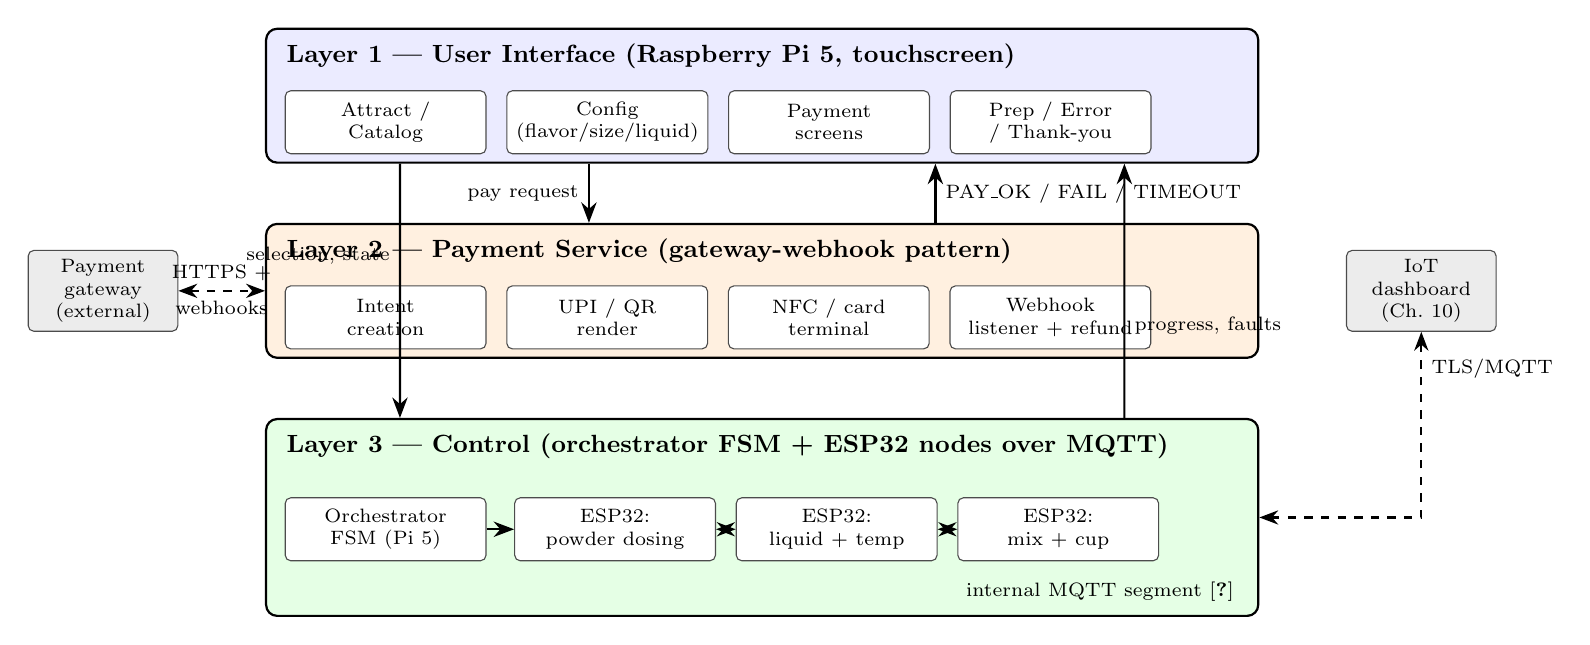
\begin{tikzpicture}[node distance=0.55cm]
  % Layer 1
  \node[layerbox, fill=blue!8] (l1) {};
  \node[anchor=north west, font=\small\bfseries] at ($(l1.north west)+(0.15,-0.08)$)
        {Layer 1 --- User Interface (Raspberry Pi 5, touchscreen)};
  \node[modbox, anchor=south west] at ($(l1.south west)+(0.25,0.12)$) (ui1) {Attract /\\Catalog};
  \node[modbox, right=0.25cm of ui1] (ui2) {Config\\(flavor/size/liquid)};
  \node[modbox, right=0.25cm of ui2] (ui3) {Payment\\screens};
  \node[modbox, right=0.25cm of ui3] (ui4) {Prep / Error\\/ Thank-you};

  % Layer 2
  \node[layerbox, fill=orange!12, below=0.75cm of l1] (l2) {};
  \node[anchor=north west, font=\small\bfseries] at ($(l2.north west)+(0.15,-0.08)$)
        {Layer 2 --- Payment Service (gateway-webhook pattern)};
  \node[modbox, anchor=south west] at ($(l2.south west)+(0.25,0.12)$) (p1) {Intent\\creation};
  \node[modbox, right=0.25cm of p1] (p2) {UPI / QR\\render};
  \node[modbox, right=0.25cm of p2] (p3) {NFC / card\\terminal};
  \node[modbox, right=0.25cm of p3] (p4) {Webhook\\listener + refund};

  % Layer 3
  \node[layerbox, fill=green!10, below=0.75cm of l2, minimum height=2.5cm] (l3) {};
  \node[anchor=north west, font=\small\bfseries] at ($(l3.north west)+(0.15,-0.08)$)
        {Layer 3 --- Control (orchestrator FSM + ESP32 nodes over MQTT)};
  \node[modbox, anchor=west] at ($(l3.west)+(0.25,-0.15)$) (c0) {Orchestrator\\FSM (Pi 5)};
  \node[modbox, right=0.35cm of c0] (c1) {ESP32:\\powder dosing};
  \node[modbox, right=0.25cm of c1] (c2) {ESP32:\\liquid + temp};
  \node[modbox, right=0.25cm of c2] (c3) {ESP32:\\mix + cup};
  \node[font=\scriptsize, anchor=south east] at ($(l3.south east)+(-0.2,0.08)$)
        {internal MQTT segment~\cite{oasis2019mqtt}};

  % External actors
  \node[modbox, fill=gray!15, left=1.1cm of l2, minimum width=1.9cm] (gw)
        {Payment\\gateway\\(external)};
  \node[modbox, fill=gray!15, right=1.1cm of l2, minimum width=1.9cm] (cloud)
        {IoT\\dashboard\\(Ch.~10)};

  % Flows
  \draw[flow] ($(l1.south)+(-2.2,0)$) -- node[left,font=\scriptsize]{pay request}
              ($(l2.north)+(-2.2,0)$);
  \draw[flow] ($(l2.north)+(2.2,0)$) -- node[right,font=\scriptsize]
              {PAY\_OK / FAIL / TIMEOUT} ($(l1.south)+(2.2,0)$);
  \draw[flow] ($(l1.south)+(-4.6,0)$) to[out=-90,in=90]
              node[left,font=\scriptsize,pos=0.35]{selection, state} ($(l3.north)+(-4.6,0)$);
  \draw[flow] ($(l3.north)+(4.6,0)$) to[out=90,in=-90]
              node[right,font=\scriptsize,pos=0.35]{progress, faults} ($(l1.south)+(4.6,0)$);
  \draw[busflow] (gw) -- node[above,font=\scriptsize]{HTTPS +}
                 node[below,font=\scriptsize]{webhooks} (l2);
  \draw[busflow] (l3.east) -| node[right,font=\scriptsize,pos=0.9]{TLS/MQTT} (cloud.south);
  \draw[flow] (c0) -- (c1);
  \draw[busflow] (c1) -- (c2);
  \draw[busflow] (c2) -- (c3);
\end{tikzpicture}
\caption{Three-layer architecture. Layers exchange a deliberately narrow
event vocabulary; the payment gateway and cloud dashboard are the only
external interfaces.}
\label{fig:threelayer}
\end{figure}

\subsection{Inter-Layer Contract}
\label{sec:contract}

Three rules govern the layers, and every chapter that follows must preserve
them:

\begin{enumerate}[label=\textbf{R\arabic*.}, itemsep=2pt]
  \item \textbf{Payment precedes actuation.} No consumable-consuming
        actuator (auger, pump, cup escapement) may run before Layer~2 has
        emitted \texttt{PAY\_OK} for the current session.
  \item \textbf{Verification precedes payment.} Layer~3 must assert
        \texttt{READY(selection)} --- cartridge level sufficient, liquid
        temperature in band, no active faults --- before Layer~1 is allowed
        to present the payment screen. This ordering is what makes automatic
        refunds rare rather than routine.
  \item \textbf{Every session terminates.} Each session ends in exactly one
        of \{\,\texttt{SERVED}, \texttt{CANCELLED},
        \texttt{REFUNDED}\,\}, and that terminal outcome is logged with the
        payment reference for reconciliation (Chapter~10).
\end{enumerate}

\section{Complete User Workflow}
\label{sec:workflow}

\subsection{Design Method}

The workflow is designed as a deterministic finite-state machine in the
statechart style~\cite{harel1987statecharts}: a finite set of states $S$, an
event alphabet $\Sigma$ (touch inputs, payment events, hardware results,
timeouts), and a transition function $\delta : S \times \Sigma \rightarrow S$
that is \emph{total} over all events that can physically occur in each state.
Designing $\delta$ to be total --- rather than leaving ``impossible'' events
undefined --- is the single most important reliability decision in the
machine: an unattended kiosk has no operator to rescue it from an unhandled
event.

Formally, a customer session is the tuple
\begin{equation}
  \mathcal{M} = (S, \Sigma, \delta, s_0, F), \qquad
  s_0 = \textsc{Idle}, \quad
  F = \{\textsc{Served}, \textsc{Cancelled}, \textsc{Refunded}\},
  \label{eq:fsm}
\end{equation}
and objective O1 requires that every reachable run of $\mathcal{M}$ ends in
$F$ within bounded time. Timeouts guarantee boundedness: every non-terminal
state carries a timeout event $\tau_s \in \Sigma$, so no state can be
occupied indefinitely.

\subsection{Narrative Walkthrough (Happy Path)}
\label{sec:happypath}

\begin{enumerate}[label=\textbf{W\arabic*.}, itemsep=2pt]
  \item \textbf{Idle / Attract.} The screen cycles promotional content and
        live prices. Any touch wakes the machine into the catalog. In the
        background, Layer~3 continuously publishes health telemetry
        (temperatures, levels, fault flags); if any \emph{blocking} fault is
        active the attract loop is replaced by an out-of-service screen.
  \item \textbf{Flavor selection.} The six cartridges are shown with live
        availability; an empty or fault-flagged cartridge renders greyed-out
        rather than being hidden (the customer should see the product exists).
  \item \textbf{Size selection.} \SI{30}{\gram} / \SI{45}{\gram} /
        \SI{60}{\gram}, with per-size pricing and macro information pulled
        from the cartridge's stored product profile.
  \item \textbf{Liquid selection.} Chilled water or refrigerated milk.
        Milk is offered only if the milk circuit's temperature log has been
        continuously in-band (Chapter~7 defines the HACCP rule that gates
        this~\cite{codexhaccp}).
  \item \textbf{Readiness check (invisible to the user).} The orchestrator
        queries Layer~3: cartridge mass $\ge$ selected dose + reserve
        margin; liquid volume sufficient; liquid temperature in
        \SIrange{4}{8}{\celsius}; cup stack non-empty; mixer and gate valve
        homed. Only on \texttt{READY} does the UI advance (rule R2).
  \item \textbf{Price confirmation and payment.} The total is displayed;
        the customer picks a rail (UPI/QR/NFC/card). Layer~2 creates a
        payment intent and the machine waits, showing a countdown
        (\SI{90}{\second} for scan-to-pay, \SI{60}{\second} for tap).
  \item \textbf{Payment confirmed.} The gateway webhook delivers capture
        confirmation; Layer~2 emits \texttt{PAY\_OK}; the orchestrator
        transitions into the locked preparation sequence (rule R1 now
        satisfied).
  \item \textbf{Preparation sequence} (detail in Chapter~4; mechanics in
        Chapters~5--8): cup drop and optical verification $\rightarrow$
        tare $\rightarrow$ gravimetric powder dose into the mixing chamber
        $\rightarrow$ liquid fill verified by mass $\rightarrow$ timed mix
        $\rightarrow$ pour/serve $\rightarrow$ nozzle rinse. The UI plays a
        stage-synchronized animation with a progress bar driven by real
        Layer-3 progress events, not a fake timer.
  \item \textbf{Serve and thank-you.} The serve window unlocks; the
        thank-you screen offers a digital receipt (QR link); after
        \SI{15}{\second} or an explicit ``Done'' the machine returns to
        \textsc{Idle} and publishes the session record to the dashboard.
\end{enumerate}

\subsection{State Inventory}
\label{sec:stateinventory}

Table~\ref{tab:states} enumerates every state with its entry action, the
events it must handle, and its timeout disposition. This table is the
normative definition; the diagram in Figure~\ref{fig:userfsm} is its
visualization.

\begin{table}[htbp]
\centering
\caption{User-workflow state inventory. Every state's event set is total;
$\tau$ denotes the state timeout.}
\label{tab:states}
\footnotesize
\begin{tabular}{@{}p{2.6cm}p{3.3cm}p{4.6cm}p{3.2cm}@{}}
\toprule
\textbf{State} & \textbf{Entry action} & \textbf{Handled events $\rightarrow$ next state} & \textbf{Timeout $\tau$} \\
\midrule
\textsc{Idle} & attract loop; poll health & touch $\rightarrow$ \textsc{Flavor}; blocking fault $\rightarrow$ \textsc{OutOfService} & --- (rest state) \\
\addlinespace[2pt]
\textsc{Flavor} & render 6 cartridges + availability & select $\rightarrow$ \textsc{Size}; back $\rightarrow$ \textsc{Idle} & \SI{45}{\second} $\rightarrow$ \textsc{Idle} \\
\addlinespace[2pt]
\textsc{Size} & render 30/45/60 g + prices & select $\rightarrow$ \textsc{Liquid}; back $\rightarrow$ \textsc{Flavor} & \SI{45}{\second} $\rightarrow$ \textsc{Idle} \\
\addlinespace[2pt]
\textsc{Liquid} & render water/milk (gated) & select $\rightarrow$ \textsc{Verify}; back $\rightarrow$ \textsc{Size} & \SI{45}{\second} $\rightarrow$ \textsc{Idle} \\
\addlinespace[2pt]
\textsc{Verify} & query Layer 3 readiness & \texttt{READY} $\rightarrow$ \textsc{Confirm}; \texttt{NOT\_READY(r)} $\rightarrow$ \textsc{SoftFault(r)} & \SI{5}{\second} $\rightarrow$ \textsc{SoftFault} \\
\addlinespace[2pt]
\textsc{Confirm} & show total, rails & rail chosen $\rightarrow$ \textsc{PayPending}; back $\rightarrow$ \textsc{Liquid}; cancel $\rightarrow$ \textsc{Cancelled} & \SI{45}{\second} $\rightarrow$ \textsc{Idle} \\
\addlinespace[2pt]
\textsc{PayPending} & create intent; show QR / arm terminal; countdown & \texttt{PAY\_OK} $\rightarrow$ \textsc{Locked\-Prep}; \texttt{PAY\_FAIL} $\rightarrow$ \textsc{PayRetry}; cancel $\rightarrow$ \textsc{Cancelled} & 60--\SI{90}{\second} = \texttt{PAY\_TIMEOUT} $\rightarrow$ \textsc{PayRetry} \\
\addlinespace[2pt]
\textsc{PayRetry} & show failure reason; offer retry / other rail & retry $\rightarrow$ \textsc{PayPending}; cancel/back $\rightarrow$ \textsc{Cancelled} & \SI{30}{\second} $\rightarrow$ \textsc{Cancelled} \\
\addlinespace[2pt]
\textsc{LockedPrep} & run W8 sequence; live progress & \texttt{PREP\_DONE} $\rightarrow$ \textsc{Served}; \texttt{PREP\_FAULT(f)} $\rightarrow$ \textsc{RefundFlow(f)} & \SI{120}{\second} hard cap $\rightarrow$ \textsc{RefundFlow} \\
\addlinespace[2pt]
\textsc{Served} & unlock window; receipt QR & done/touch $\rightarrow$ \textsc{Idle} & \SI{15}{\second} $\rightarrow$ \textsc{Idle} \\
\addlinespace[2pt]
\textsc{RefundFlow} & trigger gateway refund; show apology + ref.\ no. & \texttt{REFUND\_OK} $\rightarrow$ \textsc{Refunded}; \texttt{REFUND\_FAIL} $\rightarrow$ escalate ticket, still \textsc{Refunded} (async retry) & \SI{20}{\second} $\rightarrow$ escalate \\
\addlinespace[2pt]
\textsc{SoftFault} & explain (e.g.\ ``Vanilla temporarily out'') & acknowledge $\rightarrow$ \textsc{Flavor} & \SI{20}{\second} $\rightarrow$ \textsc{Idle} \\
\addlinespace[2pt]
\textsc{OutOfService} & fault screen + support QR; alert dashboard & fault cleared (remote/local) $\rightarrow$ \textsc{Idle} & --- (until cleared) \\
\addlinespace[2pt]
\textsc{Cancelled}$^{\dagger}$ & void intent if any & auto $\rightarrow$ \textsc{Idle} & immediate \\
\textsc{Refunded}$^{\dagger}$ & log session + refund ref. & auto $\rightarrow$ \textsc{Idle} & immediate \\
\bottomrule
\multicolumn{4}{@{}l@{}}{\scriptsize $^{\dagger}$Terminal bookkeeping states; they log and release the session, then rest in \textsc{Idle}.}
\end{tabular}
\end{table}

Two design decisions in Table~\ref{tab:states} deserve emphasis:

\begin{itemize}[itemsep=2pt]
  \item \textbf{\textsc{Verify} exists as its own state.} Readiness is
        checked \emph{after} the full selection is known (dose mass and
        liquid choice affect what ``ready'' means) and \emph{before} money
        is requested. Folding this check into \textsc{Confirm} would tempt
        race conditions; making it explicit gives it a timeout and a
        defined failure path.
  \item \textbf{\textsc{LockedPrep} ignores the touchscreen.} Once paid,
        no user input can abort or alter the sequence --- only Layer-3
        results can. This prevents the classic kiosk fault of a customer
        cancelling mid-pour and leaving the wet path in an undefined state.
\end{itemize}

\subsection{State Diagram}
\label{sec:statediagram}

\begin{figure}[htbp]
\centering
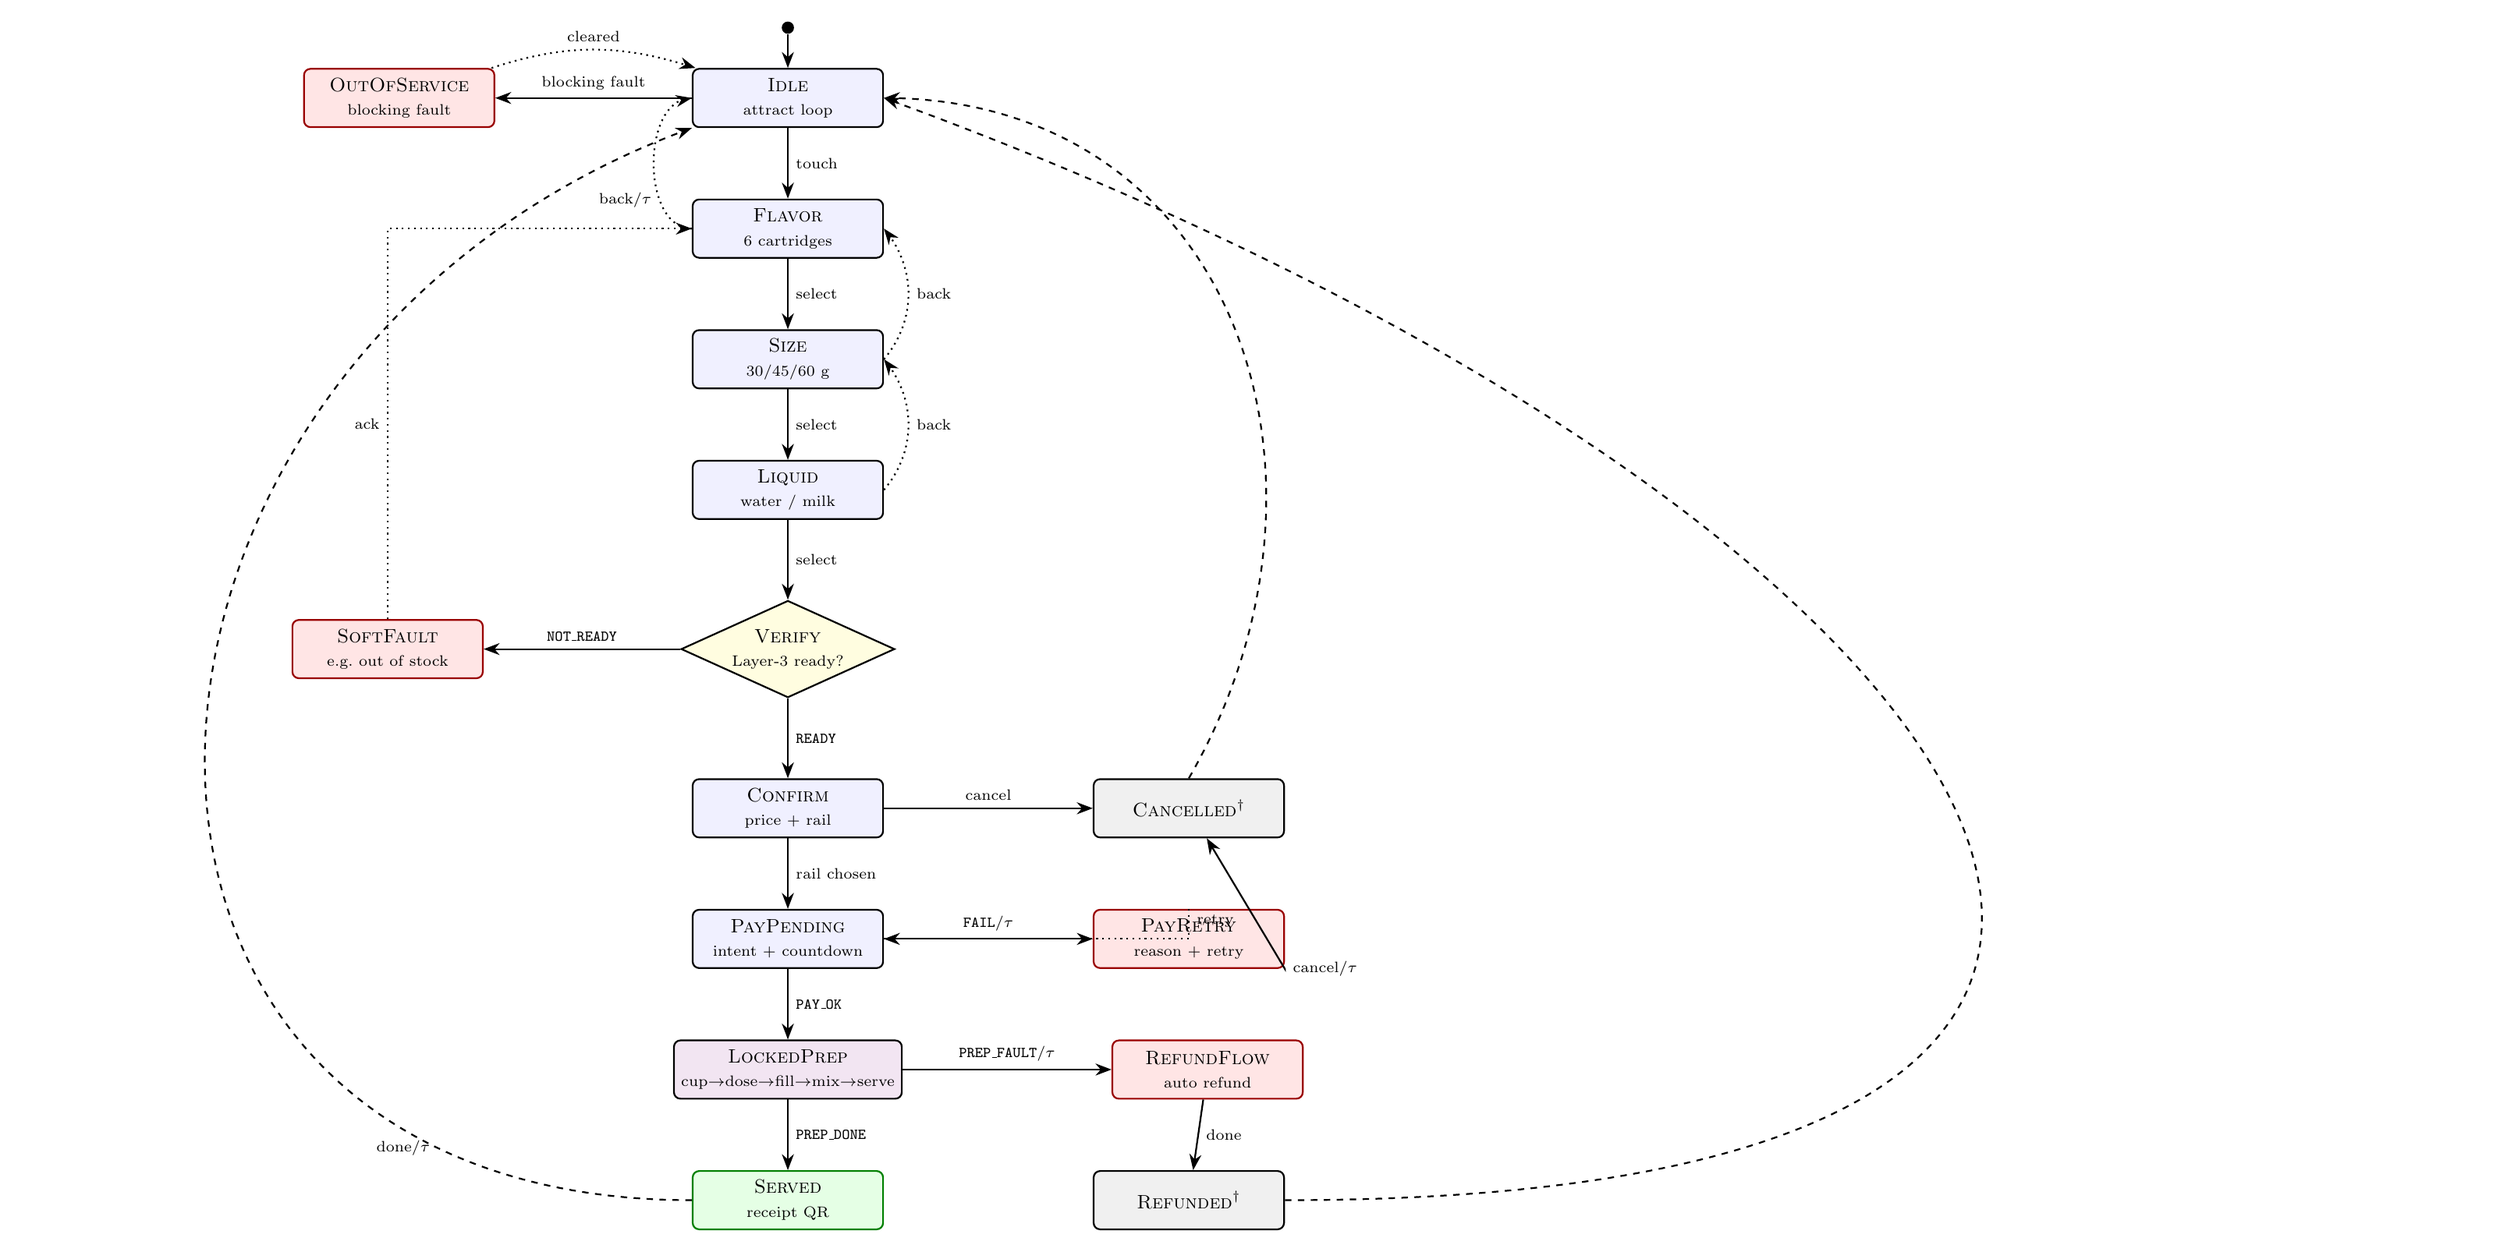
\begin{tikzpicture}[node distance=1.15cm and 1.5cm, on grid=false]
  % --- main column: selection funnel ---
  \node[sysstate] (idle) {\textsc{Idle}\\\scriptsize attract loop};
  \node[sysstate, below=of idle] (flavor) {\textsc{Flavor}\\\scriptsize 6 cartridges};
  \node[sysstate, below=of flavor] (size) {\textsc{Size}\\\scriptsize 30/45/60 g};
  \node[sysstate, below=of size] (liquid) {\textsc{Liquid}\\\scriptsize water / milk};
  \node[decision, below=1.3cm of liquid] (verify) {\textsc{Verify}\\\scriptsize Layer-3 ready?};
  \node[sysstate, below=1.3cm of verify] (confirm) {\textsc{Confirm}\\\scriptsize price + rail};
  \node[sysstate, below=of confirm] (paypend) {\textsc{PayPending}\\\scriptsize intent + countdown};
  \node[sysstate, below=of paypend, fill=violet!10] (locked)
        {\textsc{LockedPrep}\\\scriptsize cup$\to$dose$\to$fill$\to$mix$\to$serve};
  \node[okstate, below=of locked] (served) {\textsc{Served}\\\scriptsize receipt QR};

  % --- right column: payment failure handling ---
  \node[errstate, right=3.4cm of paypend] (payretry)
        {\textsc{PayRetry}\\\scriptsize reason + retry};
  \node[errstate, right=3.4cm of locked] (refund)
        {\textsc{RefundFlow}\\\scriptsize auto refund};
  \node[sysstate, right=3.4cm of served, fill=gray!12] (refunded)
        {\textsc{Refunded}$^{\dagger}$};
  \node[sysstate, right=3.4cm of confirm, fill=gray!12] (cancelled)
        {\textsc{Cancelled}$^{\dagger}$};

  % --- left column: soft fault + OOS ---
  \node[errstate, left=3.2cm of verify] (soft)
        {\textsc{SoftFault}\\\scriptsize e.g.\ out of stock};
  \node[errstate, left=3.2cm of idle] (oos)
        {\textsc{OutOfService}\\\scriptsize blocking fault};

  % --- happy path ---
  \draw[flow] (idle) -- node[right,font=\scriptsize]{touch} (flavor);
  \draw[flow] (flavor) -- node[right,font=\scriptsize]{select} (size);
  \draw[flow] (size) -- node[right,font=\scriptsize]{select} (liquid);
  \draw[flow] (liquid) -- node[right,font=\scriptsize]{select} (verify);
  \draw[flow] (verify) -- node[right,font=\scriptsize]{\texttt{READY}} (confirm);
  \draw[flow] (confirm) -- node[right,font=\scriptsize]{rail chosen} (paypend);
  \draw[flow] (paypend) -- node[right,font=\scriptsize]{\texttt{PAY\_OK}} (locked);
  \draw[flow] (locked) -- node[right,font=\scriptsize]{\texttt{PREP\_DONE}} (served);

  % --- back edges (dotted) ---
  \draw[flow, dotted] (flavor.west) to[out=180,in=180]
        node[left,font=\scriptsize,pos=0.3]{back/$\tau$} (idle.west);
  \draw[flow, dotted] (size.east) to[bend right=40]
        node[right,font=\scriptsize]{back} (flavor.east);
  \draw[flow, dotted] (liquid.east) to[bend right=40]
        node[right,font=\scriptsize]{back} (size.east);

  % --- verify failure ---
  \draw[flow] (verify) -- node[above,font=\scriptsize]{\texttt{NOT\_READY}} (soft);
  \draw[flow, dotted] (soft) |- node[left,font=\scriptsize,pos=0.25]{ack} (flavor.west);

  % --- payment branches ---
  \draw[flow] (paypend) -- node[above,font=\scriptsize]{\texttt{FAIL}/$\tau$} (payretry);
  \draw[flow, dotted] (payretry.north) |- node[right,font=\scriptsize,pos=0.2]{retry}
        (paypend.east);
  \draw[flow] (payretry) -- node[right,font=\scriptsize]{cancel/$\tau$}
        (cancelled.east |- payretry.south) -- (cancelled);
  \draw[flow] (confirm.east) -- node[above,font=\scriptsize]{cancel} (cancelled.west);

  % --- prep fault -> refund ---
  \draw[flow] (locked) -- node[above,font=\scriptsize]{\texttt{PREP\_FAULT}/$\tau$} (refund);
  \draw[flow] (refund) -- node[right,font=\scriptsize]{done} (refunded);

  % --- terminals home to idle ---
  \draw[flow, dashed] (served.west) to[out=180,in=200,looseness=1.6]
        node[left,font=\scriptsize,pos=0.15]{done/$\tau$} (idle.south west);
  \draw[flow, dashed] (cancelled.north) to[out=60,in=0,looseness=1.2] (idle.east);
  \draw[flow, dashed] (refunded.east) to[out=0,in=-20,looseness=2.6] (idle.east);

  % --- out of service ---
  \draw[flow] (idle) -- node[above,font=\scriptsize]{blocking fault} (oos);
  \draw[flow, dotted] (oos) to[bend left=18] node[above,font=\scriptsize]{cleared} (idle);

  % initial marker
  \node[circle,fill=black,inner sep=2pt, above=0.55cm of idle] (init) {};
  \draw[flow] (init) -- (idle);
\end{tikzpicture}
\caption{Complete user-workflow finite-state machine
(Eq.~\ref{eq:fsm}, Table~\ref{tab:states}). Solid edges: forward
transitions; dotted: back/retry; dashed: return-to-rest. Terminal states
($\dagger$) log the session and release to \textsc{Idle}.}
\label{fig:userfsm}
\end{figure}

\subsection{Fault Taxonomy and Refund Guarantee}
\label{sec:faults}

Faults are partitioned by \emph{when} they occur relative to payment,
because that determines the money consequence:

\begin{itemize}[itemsep=2pt]
  \item \textbf{Pre-payment (soft) faults} --- empty cartridge, liquid out
        of temperature band, cup stack empty. Handled in \textsc{Verify};
        the customer never pays. Cost: a lost sale, not a refund.
  \item \textbf{Post-payment (hard) faults} --- auger stall, load-cell
        implausibility ($>\SI{1}{\gram}$ over target with gate closed),
        pump dry-run, cup-drop failure, mix-motor overcurrent, or the
        \SI{120}{\second} sequence hard cap. Any of these raises
        \texttt{PREP\_FAULT}, the sequence is safed (valves closed, motors
        off), and \textsc{RefundFlow} issues a gateway refund against the
        original payment reference automatically. If the refund API call
        itself fails, the refund is queued for asynchronous retry and a
        dashboard ticket is raised --- the customer still sees a refund
        confirmation with a reference number.
  \item \textbf{Blocking faults} --- refrigeration failure, repeated dosing
        faults on all cartridges, door-open interlock. These take the whole
        machine to \textsc{OutOfService} until cleared locally or remotely
        (Chapter~11 formalizes the interlock logic).
\end{itemize}

The refund guarantee of objective~O4 follows structurally: money is captured
only in \textsc{PayPending}$\rightarrow$\textsc{LockedPrep}, and
\textsc{LockedPrep} has exactly two exits --- \textsc{Served} or
\textsc{RefundFlow}.

\subsection{Cycle-Time Budget}
\label{sec:timing}

Objective O3 caps the paid-to-served time at \SI{60}{\second}. The budget
is allocated per stage as
\begin{equation}
  T_{\text{cycle}} = t_{\text{cup}} + t_{\text{tare}} + t_{\text{dose}}
                   + t_{\text{fill}} + t_{\text{mix}} + t_{\text{serve}}
                   + t_{\text{margin}},
  \label{eq:cycle}
\end{equation}
with nominal allocations (worst case = \SI{60}{\gram} dose, \SI{400}{\milli\litre} fill):
\begin{equation}
  T_{\text{cycle}} \approx
  \underbrace{3}_{\text{cup}}
  + \underbrace{2}_{\text{tare}}
  + \underbrace{12}_{\text{dose}}
  + \underbrace{10}_{\text{fill}}
  + \underbrace{20}_{\text{mix}}
  + \underbrace{5}_{\text{serve}}
  + \underbrace{8}_{\text{margin}}
  = \SI{60}{\second}.
  \label{eq:cyclebudget}
\end{equation}
Each allocation becomes a derived requirement on its subsystem: the dosing
stage must sustain an average feed rate of at least
$\SI{60}{\gram}/\SI{12}{\second} = \SI{5}{\gram\per\second}$ \emph{including}
its slow-approach fine-dosing phase (Chapter~6 derives the auger
coarse/fine speed profile from this number), and the fill stage requires a
pump delivering $\ge \SI{2.4}{\litre\per\minute}$ at the nozzle (Chapter~7).
The \SI{120}{\second} hard cap in Table~\ref{tab:states} is deliberately
$2\times$ the nominal budget: it trips only on genuine faults, never on
normal variation.

\section{Operational Modes}
\label{sec:modes}

Beyond the customer session, the machine runs three additional top-level
modes, each a sibling statechart entered from \textsc{Idle}:

\begin{description}[itemsep=2pt]
  \item[Admin mode (Chapter 2).] PIN-protected on-screen entry: price
        editing, cartridge assignment after restock, manual jog of each
        actuator, log review, and forced cleaning cycle.
  \item[Cleaning mode (Chapters 7--8, 11).] Post-serve rinse is automatic
        inside \textsc{LockedPrep}; the scheduled deep-clean (mixer, nozzle,
        milk line purge) runs at a configured off-peak time and takes the
        machine out of service for its duration, logged for HACCP
        records~\cite{codexhaccp}.
  \item[Maintenance/OTA mode (Chapter 10).] Remote firmware/UI updates are
        accepted only in \textsc{Idle} with no session active; the machine
        shows a brief updating screen and self-verifies before returning to
        service.
\end{description}

\section{Chapter Summary and Thesis Organization}
\label{sec:organization}

This chapter fixed the machine's requirements (P1--P5), objectives (O1--O5,
S1--S4), the three-layer architecture with its inter-layer rules (R1--R3),
and the complete user workflow as a total finite-state machine
(Eq.~\ref{eq:fsm}, Table~\ref{tab:states}, Fig.~\ref{fig:userfsm}) with a
quantitative cycle-time budget (Eq.~\ref{eq:cyclebudget}) that seeds derived
requirements for the subsystem chapters. The remainder of the thesis expands
each element: Chapter~2 the touchscreen UI, Chapter~3 the payment gateway
integration, Chapter~4 the control state machine and orchestrator code,
Chapters~5--8 the mechanical, dosing, thermal, and mixing/dispensing
hardware, Chapter~9 the electronics and PCB, Chapter~10 the embedded
software and IoT dashboard, Chapter~11 safety and HACCP, Chapter~12
manufacturing and cost, and Chapter~13 the consolidated references and
appendices.

% \input{chapter2}   % Touchscreen UI
% \input{chapter3}   % Payment Gateway
% \input{chapter4}   % Control System State Machine
% \input{chapter5}   % Mechanical Design & Cartridge System
% \input{chapter6}   % Precision Powder Dispensing
% \input{chapter7}   % Refrigeration & Milk System
% \input{chapter8}   % Mixing Chamber & Cup/Nozzle Dispensing
% \input{chapter9}   % Electronics & PCB
% \input{chapter10}  % Embedded Software & IoT Dashboard
% \input{chapter11}  % Safety, HACCP, Reliability
% \input{chapter12}  % Manufacturing, BOM, Cost
% \input{chapter13}  % References compilation & Appendices

% ---------- Bibliography (grows as chapters cite; IEEE style) ----------
\bibliographystyle{IEEEtran}
\bibliography{references}

\end{document}
